
%%%%%%%%%%%%%%%%%%%%%%% xxxxxxxxxxxxxxxx %%%%%%%%%%%%%%%%%%%%%%%%%
%
%	copyright by Springer Heidelberg
%   http://www.springer.com/lncs       Springer Heidelberg 2006/05/04
%
%
%%%%%%%%%%%%%%%%%%%%%%%%%%%%%%%%%%%%%%%%%%%%%%%%%%%%%%%%%%%%%%%%%%%


\documentclass[runningheads,a4paper]{llncs}

\usepackage{amssymb}
\setcounter{tocdepth}{3}
\usepackage{graphicx}
\usepackage{caption}
\usepackage{url} %takes care of proper line breaks for URLs
\usepackage{hyperref} % creates clickable links and references.
\usepackage{float}% exact position of figures
\setlength{\parindent}{0pt} % no indent on new paragraphs


\begin{document}

\mainmatter  % start of an individual contribution

% first the title is needed
\title{Domain Specific Modeling}

% a short form should be given in case it is too long for the running head
\titlerunning{Lecture Notes in Computer Science: Authors' Instructions}


\author{Tim Schneider\\ tim-1.schneider@uni-ulm.de}
\institute{Institute of Databases and
Information Systems, Ulm University}


\maketitle


\begin{abstract}
%The abstract should summarize the contents of the paper and should
%contain at least 70 and at most 150 words. It should be written using the
Nowadays computers and smartphones make it easier for both novices and domain experts to build 
and explore their own models and learn new scientific ideas in the process.
Domain Specific Modeling can support both experts and novices in building models for different domains.
There are approaches (e.g. LEGO Mindstorms,Starlogo) which enable novices with few or even no programming 
skills to implement their own models.
Domain Experts on the other hand may use modeling languages (e.g. SimuLink,BPMN) designed for a domain to create models, 
which allow them to focus on domain-specific problems instead of implementation-specific details like supported 
language features of a programming language.
In this paper we will give an overview over different domain-specific modeling langues with a focus on modeling languages for novices
as well as describe features offered by Xtext and GMF (from the Eclipse Modeling framework) supporting the creation of textual and graphical modeling languages.
\end{abstract}

\section{Introduction}
\label{sec:introduction}
For centuries people from da Vinci to Einstein have created models to help them better 
understand patterns and processes in the world around them. 
Nowadays computers and smartphones make it easier for both novices and domain experts to build 
and explore their own models and learn new scientific ideas in the process.
Domain Specific Modeling can support both experts and novices in building models for different domains.
There are approaches (e.g. LEGO Mindstorms,Starlogo) that enable novices with few or even no programming 
skills at all to implement their own models.
Domain experts on the other hand may use modeling languages (e.g. SimuLink,BPMN) designed for a specific domain to create models, 
which allows them to focus on domain-specific problems instead of implementation-specific details like supported 
language features of a general pupose programming language (e.g. C,C++,Java).
In this paper we will give a an overview about domain specific modeling languages for novices.
Additionally we will present the tools Xtext and GMF for creating textual and graphical modeling languages. 

% \begin{itemize}
%  \item can help experts and novices builing Models for different domains
%  \item enables novices with few or even no programming skills at all to implement their own models (e.g. MindStorm,Starlogo)
%  \item supports domain experts by setting focus on the domain-specific problems (e.g. SimuLink,BPMN)
%   \end{itemize}

\subsection{Foundation}
\label{subsec:introduction}
Before speaking about domain specific modeling languages we will give some short definitions for the  
terms \emph{model} and \emph{domain}.

\subsubsection{Model}
% \begin{itemize}
%  \item What is a model? (Definition  [Stachowiak]
%  + some Explanation)
%  \item Abstraction: Remove details which do not serve the purpose
% 
%  \item Homomorphism: Statements on model elements hold for real world entities
%  \item Pragmatics: Model has some purpose
%  \item + example (novice) house Made of LEGOS $\rightarrow $ Model for a ``real'' house / building
%  \item + example (expert) blueprints from an architekt $\rightarrow $ different model, but  represents same object in real 
%  world
%  
%  \item Abstraction brings representational bias 
%  \item $\rightarrow$ electric cable installations, water pipes cannot be ``expressed'' in lego but they can with blueprints
%  \item $\rightarrow$ lego allows 3D Modeling while Blueprints cannot (oonly via 2d projections/ optical illusions)
%  \end{itemize}
%  
  When speaking about domain specific modeling languages, we need to define what a model is:
  
  \begin{quote}
   A model is a formal representation of entities and relationships in the real world (abstraction) 
  with a certain correspondence (homomorphism) for a certain purpose (pragmatics) \cite{stachowiak1973allgemeine}.
  \end{quote}
  
  This definition contains three aspects: abstraction, homomorphism, pragmatics.
  A model should create a simplified view on the represented entities and relationships and 
  only contain details which are relevant (abstraction).
  Additionally statements on the model elements should hold for the represented entities and relationships (homomorphism).
  The question which details are relevant and should be included in the model is determined by the purpose of a model (pragmatics).  
 
  Creating models is something we do in our everday lifes:
  When building a house in LEGO a child creates a model which serves as a representation of building in the real world.
  It is a simplified view on the original as it abstracts from detais like used materials, installed cables and water pipes and focusses
  on the shapes of the building.
  Another example for creating models is an architekt, who creates blueprints for some house, serving as a model for it.
  Blueprints contain 2D projections of walls and installations in that house from different viewpoints and abstract from the original by ommiting
  details like materials and some 3D information. 
  We can see from this example that these abstraction also brings a representational bias:
  Electric cable installations and water pipes cannot be modeled in LEGO but they can with blueprints.
  LEGO models on ther other hand allows to model structures directly in 3D while blueprints cannot.
  
\subsubsection{Domain}
  
  Although novices (e.g. the child) and experts(e.g. the architect) may have different views on the same thing (e.g. the house)
  they share a common understanding in the concepts of the real world: 
  Both of them know that the concepts ``wall'' and ``roof'' are related to parts of a building and that a house needs both to be a valid house.
  These common knowledge of the requirements, concepts and functionality in a field of study is refered to as a domain (e.g. architecture). 
  
%  \begin{itemize}
%  \item novice and expert have different views on the same thing  but use different models / languages
%  \item both models may be used in the context of a domain (Architekture)
%  \item What is a Domain? (Definition + some Explanation)
%  \end{itemize}
  
 \subsection{Domain Specific Modeling Languages}
 Domain specific languages are modeling languages, designed to create models representing entities and relationships of a certain domain,
 containing textual or graphical representations of relevant concepts from that domain. The pupose of a domain specific modeling languages
 is to support users in building models from a specific domain.
 
 There are two kinds of modeling languages, which are used in these tools to create models:
 \emph{Graphical Modeling Languages} use graphical shapes and
 \emph{Textual Modeling Languages} use text to represent entities and relationships from the real world.
 The same model may be expressed in both, a graphical or textual modeling languages.
 
 A finite state machine for example can be represented as a set of nodes, labeled boxes and arrows, while it can also be 
 represented by a textual description following a grammar to represent the same finite state machine.
 
  \begin{figure}[H]
      \centering
      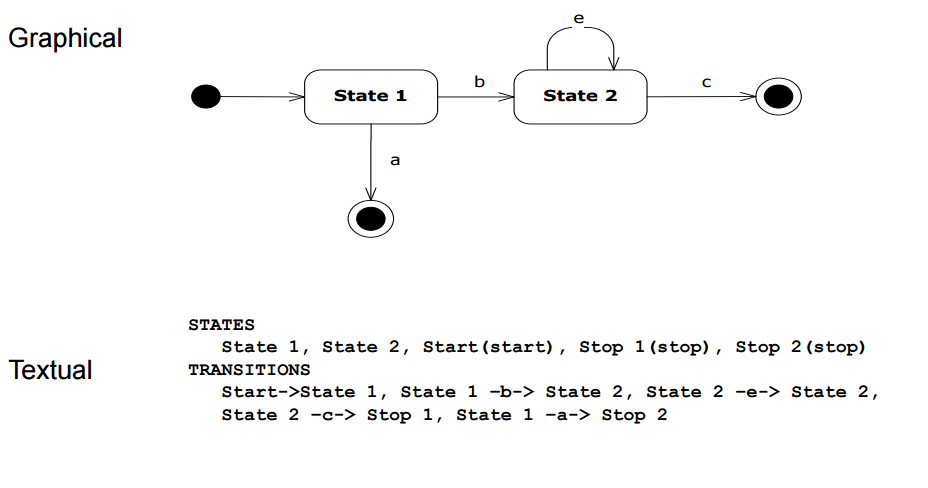
\includegraphics[width=\textwidth]{images/GraficalTextualComparison.PNG}
      \captionof{figure}{comparison between textual modeling language and graphcal modeling language for the same model}
      \label{compare:textgraphiclang}
    \end{figure}

 Users have different levels of expertise in a domain: a Software-Engineer has a more detailed knowledge in the computer science domain as a medical doctor.
 We will therefore distinguish between domain experts and novices and focus on domain specific languages for novices in this paper.
 
%  \begin{itemize}
%  \item different approaches :  Graphical Modeling Languages, Textual Modeling Languages
%  \item 
%    \begin{figure}[ht]
%       \centering
%       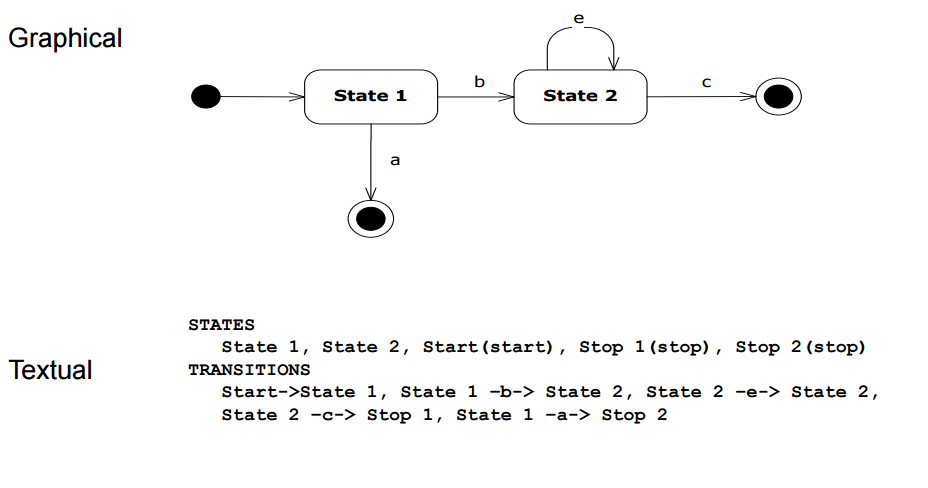
\includegraphics[width=\textwidth]{images/GraficalTextualComparison.PNG}
%       \captionof{figure}{comparison between textual modeling language and graphcal modeling language for the same model}
%     \end{figure}
%  
%  \item examples (domain experts): BPMN , SimuLink
%  \item examples (novice ): STARLOGO 
%  \end{itemize}
 
 \section{Domain Specific Modeling Languages for Novices}
 As there is a variety of software tools available, which implement different modeling languages, this section will give an overview 
 about modeling languages designed to support novices with few or even no programming languages in creating models and help them better 
 understand patterns and processes in the world around them.
 
 \subsection{StarLogo TNG}
  %enable students to build simulations and learn features of complex systems without extensive background knowledge (Klopfer et al., 2009a; 2009b)
  %provides an environment for building agent-based models
  StarLogo is a client based modeling software, developed specifically to enable students to 
  create models for the simulation of complex systems without extensive programming skills \cite{klopfer2009starlogo}.
  It provides a graphical modeling language using blocks instead of a textual syntax. 
  These blocks are coloured based on the function they have in the program and their shapes only allow syntactically correct constructs \cite{klopfer2009starlogo}.
  This eases the learning of basic programming concepts such as control-flow (e.g. loops, if-then statements),
  assignments and methods by providing intuitive graphical mappings. Since StarLogo TNG uses these puzzle-piece shapes, understanding 
  control-flow, for example, ``requires little more than visually parsing the if or repeat commands 
  Figure \ref{fig1} to conclude that items placed within the then slot will be performed if the items placed within the 
  test slot are true, or the items placed within the do slot will be subject to the number of repetitions placed within the times slot''\cite{smith2011biology}.
  Using puzzle-piece shapes for basic programming concept avoids syntactic errors, 
  which are one of the main difficulties in learning textual programming languages.
  Figure \ref{fig1} shows an exmaple for the blocks used by StarLogo TNG : 
  the curved shape of a Boolean variable is easy to distinguish from the pointed shape of a number value.
  
  \begin{figure}[H]
	\centering
  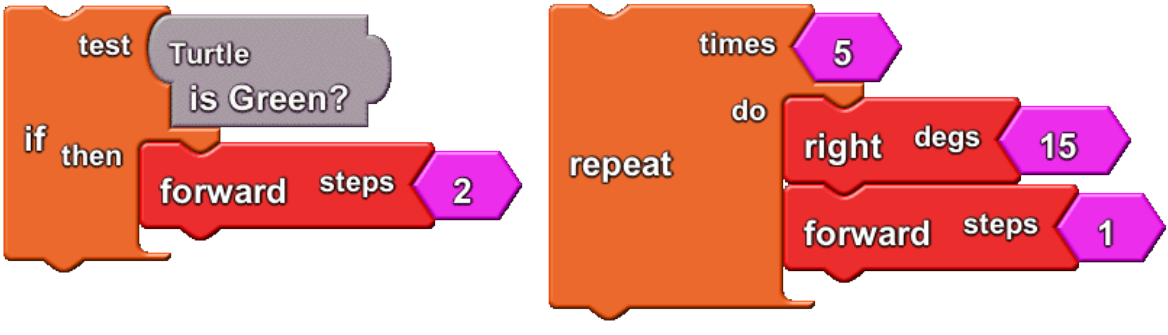
\includegraphics[width=0.5\textwidth]{images/StarLogoTNGBlocksEx.PNG}
	\caption{ StarLogo TNG’s graphical programming blocks. Example if (left) and repeat (right) blocks are shown. The
	  if block commands a Turtle agent to take two steps forward if it is green; the repeat block commands an agent to
	  repeat five times the sequence of turning right 15 degrees and taking one step forward. (from \cite{smith2011biology})}
	\label{fig1}
  \end{figure}
  
  %   \begin{itemize}
%   \item is a client-based modeling and simulation software
%   \item enables secondary school students and teachers to model decentralized systems through agent-based programming
%   \item facilitates the creation and understanding of simulations of complex systems
%   \item graphical programming blocks instead of text-based computer code
%   \end{itemize}

   \subsection{Snatch}

  \begin{itemize}
  \item Graphical Modeling Language (similar to StarLogo)
  \item developers goal: ``make it easy for everyone,
of all ages, backgrounds, and interests, to program
their own interactive stories, games, animations, and
simulations, and share their creations with one another''
  \end{itemize}
    \begin{figure}[H]
      \centering
      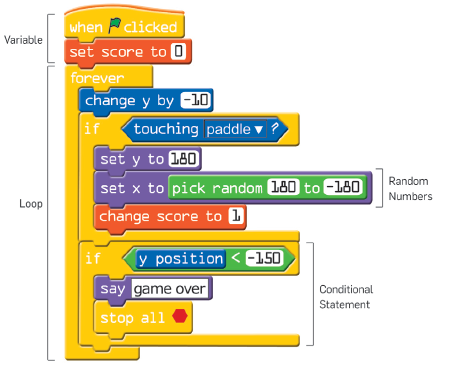
\includegraphics[width=\textwidth]{images/Snatch1.PNG}
      \captionof{figure}{Sample Scratch script (from Pong-like paddle game) highlighting computational
and mathematical concepts}
    \end{figure}
  
  
  \subsection{PhyDSL}
  Both StarLogo and Snatch use graphical modeling languages for creating models. 
  \emph{PhyDSL} is a tool, designed as an Eclipse\cite{eclipse} plugin that uses a textual modeling language for creating models for the game development domain.
  It was designed for the purpose of supporting the fast prototyping of physics-based games, including platform, shoot ’em up, 
  puzzle and maze games \cite{guana2014phydsl}. 
  The provided frontend includes a text editor (including syntax highlighting and text completion), which is used to define gameplay in highlevel
  terms describing the gameplay static, dynamic elements and their behaviors by a domain specific language.  
  It is based on the \emph{Eclipse Modeling Framework}\cite{} (EMF) and uses codegeneration for deriving C\# code supported by Microsoft’s
  DirectX API. 
  The modeling language provided by PhyDSL consists of four gameplay definition sections: mobile and
  static actor definition (Fig. \ref{actordef}), 
  environment and layout definition (Fig. \ref{envdef}), 
  activities definition (Fig. \ref{activitiesdef}), 
  and scoring rules definition (Fig. \ref{rulesdef}).
  
%  \begin{itemize}
%   \item textual modeling for (simple) game dev domain
%   \item based on EMF
%   \item allows codegeneration from the created models
%   \item mobile gameplay definition sections:
%     \begin{itemize}
%     \item static actor definition
%     \item environment and layout definition
%     \item activities definition
%     \item scoring rules definition
%     \end{itemize}
%   
%   \end{itemize}
\begin{minipage}{\textwidth}
     \begin{figure}[H]
      \centering
      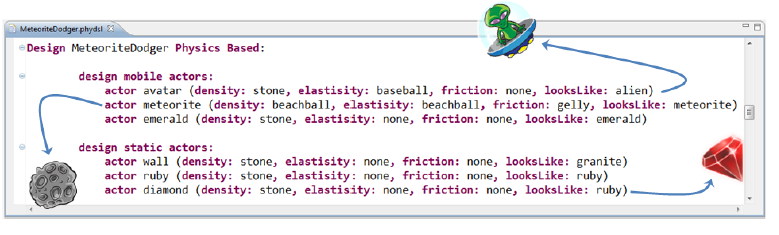
\includegraphics[width=\textwidth]{images/PhyDSL1.PNG}
      \captionof{figure}{PhyDSL: static actor definition (from  \cite{guana2014phydsl})}
      \label{actordef}
    \end{figure}
      \begin{figure}[H]
      \centering
      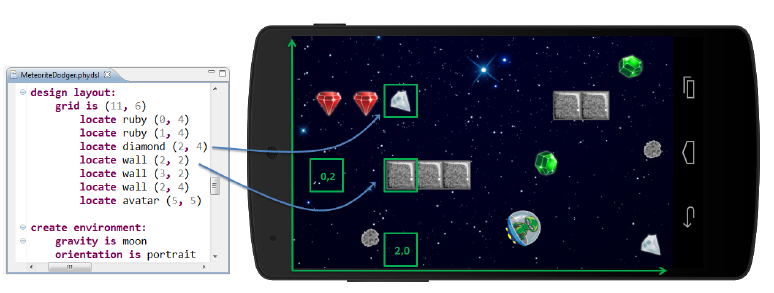
\includegraphics[width=\textwidth]{images/PhyDSL2.PNG}
      \captionof{figure}{PhyDSL: environment and layout definition(from  \cite{guana2014phydsl})}
      \label{envdef}
    \end{figure}
  \begin{figure}[H]
      \centering
      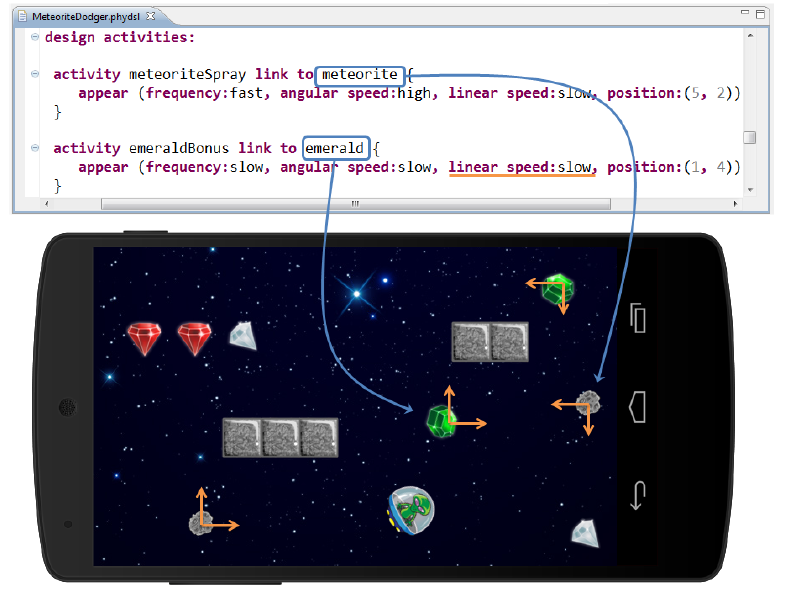
\includegraphics[width=\textwidth]{images/PhyDSL3.PNG}
      \captionof{figure}{PhyDSL: activities definition(from  \cite{guana2014phydsl})}
      \label{activitiesdef}
    \end{figure}
  \end{minipage}

\begin{figure}[H]
      \centering
      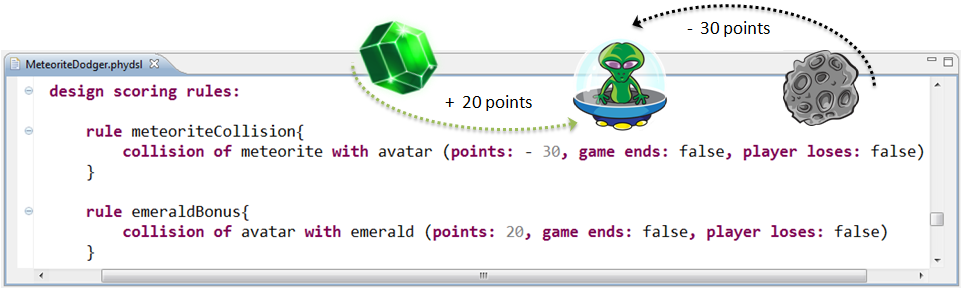
\includegraphics[width=\textwidth]{images/PhyDSL4.PNG}
      \captionof{figure}{PhyDSL - Scoring Rule Definition for Collision Rules (from  \cite{guana2014phydsl})}
      \label{rulesdef}
    \end{figure}

   \pagebreak
   
   \subsection{LEGO Mindstorms}
   Another example for a graphical modeling language made for novices is the EV3 Programmer App
   for LEGO Mindstorms which includes a block-based graphical modeling langue for creating programms
   for the LEGO MindStorm Robots. Programs are loaded and executed on a EV3 P-brick \ref{ev3pbrick}, 
   which offers input and output connections for interaction with sensors and actuators.
   Different colors are used to indicate wether a blocks triggers some action (green), is used for flow control (orange),
   reads data from some input (e.g. color sensor)(yellow) or trigger some data operation (e.g. read/write some variable).
   
%   \begin{itemize}
%   \item EV3 Programmer App or Computer Software for programming lego robots in a graphical syntax 
%   \item action blocks (green), flow blocks (orange), sensor blocks (yellow), data operation blocks (red), advanced blocks (dark blue)
%   \item programms are executed on the EV3 P-brick. 
%   %https://www.lego.com/en-us/mindstorms/learn-to-program
%   \end{itemize}
  
  \begin{minipage}{.5\textwidth} %
	  \centering
    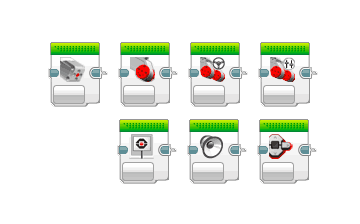
\includegraphics[width=\textwidth]{images/LearnToProgram_action_blocks_landscape.png}
	  \captionof{figure}{The action blocks control the actions of the program, e.g. motor rotations, image, sound and the light on the EV3 P-brick.}
  \end{minipage} %
  \begin{minipage}{.5\textwidth} %
	  \centering
    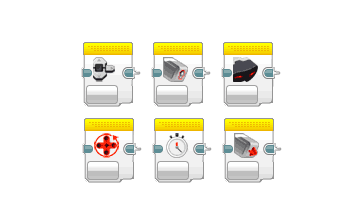
\includegraphics[width=\textwidth]{images/LearnToProgram_sensor_blocks_landscape.png}
	 \captionof{figure}{The sensor blocks allow to read the inputs e.g. from a color sensor, IR sensor, touch sensor.}
  \end{minipage}
  \begin{minipage}{.5\textwidth} %
	  \centering
    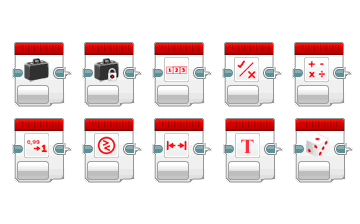
\includegraphics[width=\textwidth]{images/LearnToProgram_operations_blocks_landscape.png}
    \captionof{figure}{The data operation blocks let the user write and read variables, compare values for example.}
  \end{minipage}
  \begin{minipage}{.5\textwidth} %
	  \centering
    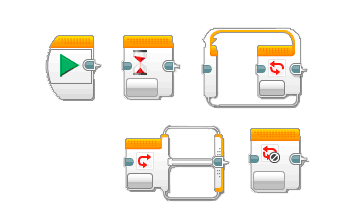
\includegraphics[width=\textwidth]{images/LearnToProgram_flow_blocks_landscape.png}
    \captionof{figure}{The Flow blocks control the flow of the program.}
    \label{ev3pbrick}
  \end{minipage}
  
  
    \begin{figure}[ht]
	  \centering
    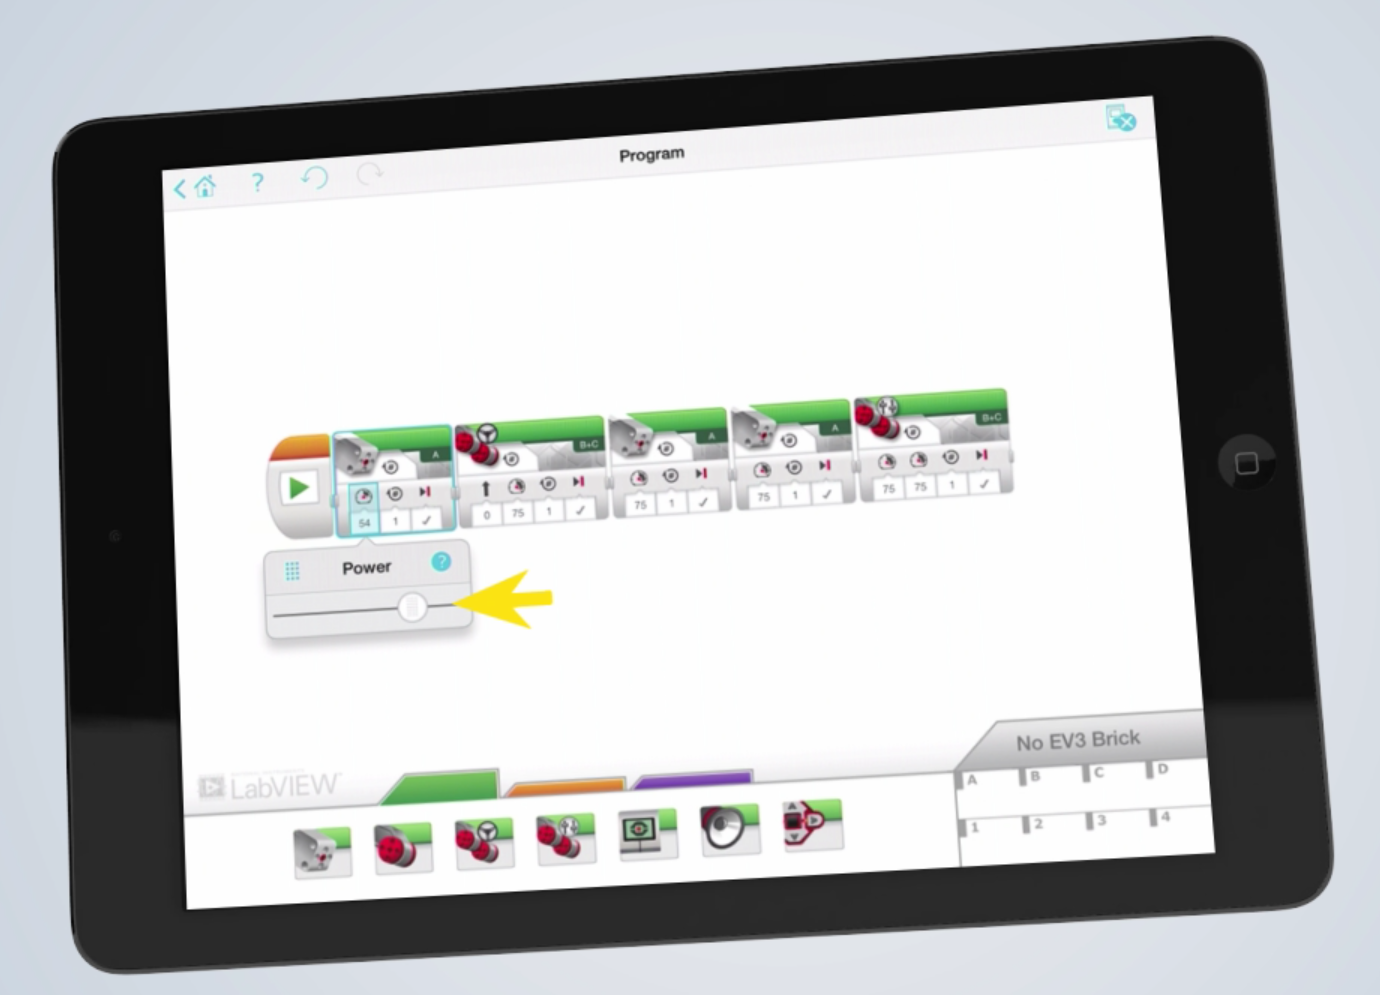
\includegraphics[width=0.5\textwidth]{images/mindstorms0.PNG}
	  \caption{EV3 Programmer App on a tablet used to create programms using a graphical modeling language}
    \end{figure}

    \subsection{Sensr}
    \begin{itemize}
     \item enables people without programming skills to build mobile data collection and management tools for citizen science
    \end{itemize}

    
    \section{Creating Domain Specific Modeling Languages}
    Domain Specific Modeling Languages are implemented in various software tools using textual or graphical modeling languages.
    In fact, there are approaches to define these modeling languages as models using some kind of meta-language.
    Xtext and GMF are implementions from the Eclipse Modeling Framework (EMF), which adopt this approach.
    
    \subsection{Ecore}
    Xtext and GMF use a 
    \begin{itemize}
	\item  a meta model  for describing models and runtime support for the models .
    \end{itemize}
    
    \subsection{Xtext}
    Xtext is a framework for development of programming languages and domain specific modeling languages \cite{eysholdt2010xtext}.
    It uses a syntax similar to extended backus\–naur form (EBNF) to describe custom textual modeling languages. 
    From this modeling language definition Xtext generates a custom Text-Editor for Eclipse whose features include code-completion and syntax-highlighting
    as well as a parser for parsing models from text files specified in the defined grammar. This makes it easy for experts of the language design
    domain to create models for custom modeling languages without programming skills or knowledge on how to implement a parser.
    As the modeling language definitions are stored in the Ecore format, other tools in the EMF framework can process data from the parsed 
    models (e.g. Acceleo\cite{musset2006acceleo} for performing codegeneration).  
    
    \begin{figure}[H]
      \centering
      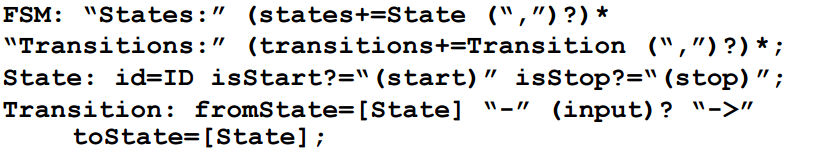
\includegraphics[width=\textwidth]{images/XTextGrammar.PNG}
      \captionof{figure}{Xtext grammar of a textual modeling language for finite state machines. 
      Figure \ref{compare:textgraphiclang} contains an textual description of a state machine 
      which follows this grammar definition.}
    \end{figure}
   
%     \begin{itemize}
%       \item used to create textual DSLs for ecore (meta-)models designed in EMF
%       \item syntax similar to EBNF
%       \item one rule for each (meta-)model element
%     \end{itemize}
%     
    \subsection{GMF}
     \begin{itemize}
     \item used to create graphcal DSLs for  models described in Ecore
     \item connects domain model and a graphical model via mapping modell
    \end{itemize}
    
    \begin{figure}[ht]
      \centering
      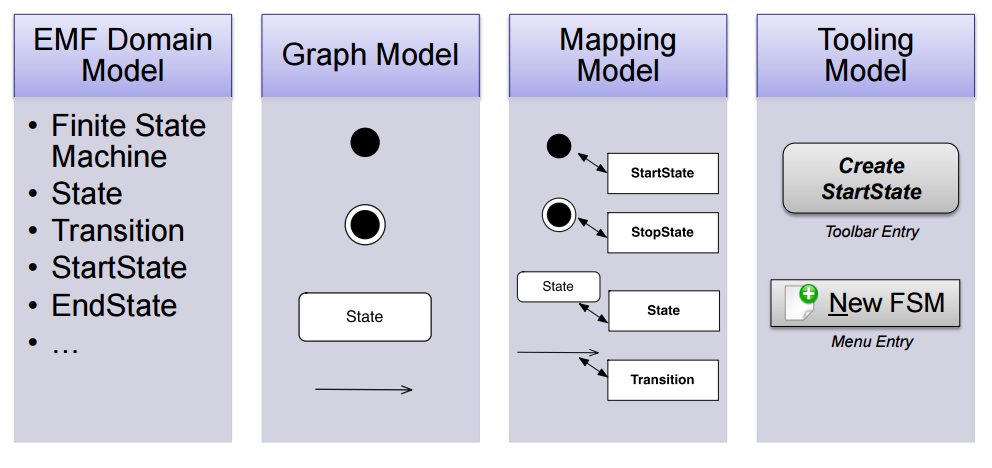
\includegraphics[width=\textwidth]{images/TableGMFSteps.PNG}
      \captionof{figure}{}
    \end{figure}

\section{Summary}\label{sec:summary}
\begin{itemize}
 \item DSM allows novices to build and explore 
their own models and learn new scientific ideas in the process
\item domain experts are supported by setting focus on domain specific problems
\end{itemize}

  
% 
% ---- Bibliography ----
% 
\nocite{*}

\bibliographystyle{splncs}
\bibliography{citations}
\end{document}

